\section{Linear Time Invariant Systems and Controls}

There is a branch of controls called Linear Time Invariant (LTI)
Systems that is often taught at the undergraduate level. Although
almost every system encountered in standard applications whether
aerospace or not are non-linear, it is still beneficial and more
simple to learn about control system dynamics when the system
parameters are constant and linear. 

\subsection{Linear Dynamics}

Standard nonlinear dynamics can be placed into standard
nonlinear affine form as shown below after much simplification of
terms
\begin{equation}
  \dot{\vec{x}} = \vec{f}(\vec{x}) + \vec{g}(\vec{x})\vec{u}
\end{equation}
where $\vec{u}$ is the control input which could be the forces and
moments from reaction wheels or thrusters for a spacecraft or lift and drag for an airplane. The vectors $f$ and $g$ represent the systems dynamics which is dependent on the system itself. Note that if the dynamics cannot be put into affine form, the system is highly nonlinear and the control system designed for that would require more sophisticated analysis like Lyapunov design or sliding mode control. That will be discussed in a later section. For the affine form however, the equation can be
linearized to give the equation below. 
\begin{equation}
  \Delta \dot{\vec{x}} = {\bf A}\Delta {\vec{x}} + {\bf B}\Delta \vec{u}
\end{equation}
where $\Delta \vec{x} = \vec{x} - \vec{x}_e$ and $\vec{x}_e$ is an
equilibrium point. In this formulation ${\bf A} = \partial \vec{f}/\partial \vec{x}$. and 
${\bf B} = \partial \vec{g}/\partial \vec{x}$ which are partial derivatives of the state matrices.

\subsection{General Formulation of Differential Equations}

The linear systems of equations derived above are in state space form. That is the vector $\vec{x}$ contains all the states of the system. However, it is often easier to understand the dynamics of a system when it is in the form of a single differential equation with all states and derivatives shown in the same equation. Practical examples also help the undergraduate controls engineer as math with practical context is the best way to learn in my humble opinion. The sections below will discuss first and second order systems which are the most common types of systems encountered in engineering applications. Note that higher order systems can be reduced to first and second order systems by using techniques such as root locus or pole placement since higher order systems typically have high frequency dynamics that can be ignored for control purposes. For the most part, first and second order systems are all that is needed to understand the basics of control systems and represent the majority of systems encountered in practice.

\subsubsection{First Order Systems}

A first order system undergoing free motion will have dynamics that look like this
\begin{equation} \label{e:first_order}
\dot{q} + \sigma q = \sigma f
\end{equation}
\noindent where q is a generalized coordinate, $\sigma$ is the inverse of the time constant $\tau$, and f is the forcing function. Examples of these types of systems in include thermistors, servos, and velocity equations for system dynamics. 

\subsubsection{Second Order Systems}

A second order system undergoing free motion will have dynamics that look like this
\begin{equation}\label{e:second_order}
\ddot{q} + 2\zeta \omega_n \dot{q} + {\omega_n}^2 = {\omega_n}^2 f
\end{equation}
where $q$ is a generalized coordinate, $\sigma$ is the inverse of the time constant $\tau$, f is the forcing function, $\omega_n$ is the natural frequency of the system and $\zeta$ is the damping ratio. Examples of these types of systems include mass, spring dampers in linear translation as well as torsional systems and penduluums. Anything that oscillates will exhibit this behavior. 

\subsection{Equation of Motion Formulation for Practical Systems}

The sections below will discuss practical examples of first and second order systems. Many of these examples are classic examples found in many dynamics and controls textbooks and ones that I typically teach budding control systems aerospace/mechanical engineers. Each one offers a slightly different set of dynamics and challenges that will help the undergraduate controls engineer understand the concepts of linear systems as well as how to control them and also determine stability. 

\subsubsection{Velocity of a Car}

Consider a car moving in one dimension. The primary forces acting on the car are the driving force from the tires, $F$, and a linear viscous drag force, $D = -cv$, where $c$ is the viscous drag coefficient and $v$ is the velocity of the car.
\begin{figure}[H]
    \centering
    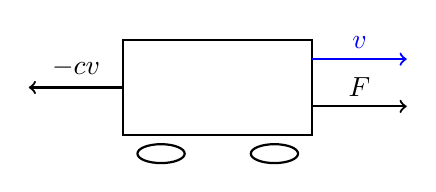
\begin{tikzpicture}[scale=1.2]
        % Draw the car as a rectangle
        \draw[thick] (0,0) rectangle (2,1);
        % Wheels
        \draw[thick] (0.4,-0.2) ellipse (0.25 and 0.1);
        \draw[thick] (1.6,-0.2) ellipse (0.25 and 0.1);
        % Forces
        \draw[->,thick] (2,0.3) -- ++(1,0) node[midway, above] {$F$};
        \draw[->,thick] (0,0.5) -- ++(-1,0) node[midway, above] {$-cv$};
        % Velocity arrow
        \draw[->,thick,blue] (2.0,0.8) -- ++(1,0.0) node[midway, above] {$v$};
    \end{tikzpicture}
    \caption{Free body diagram of a car}
    \label{f:car_fbd}
\end{figure}
\noindent Applying Newton's second law, the sum of forces is equal to mass times acceleration:
\begin{equation}
  m\dot{v} = F - cv
\end{equation}
where $m$ is the mass of the car, $F$ is the force generated by the tires, and $-cv$ is the linear drag. In this case to make the system first order we simply leave acceleration as $\dot{v}$ instead of $\ddot{x}$ where x would be the position of the vehicle. Rearranging, we obtain the standard first-order linear differential equation:
\begin{equation}
  \dot{v} + \frac{c}{m}v = \frac{F}{m}
\end{equation}
This equation describes the velocity dynamics of the car under a linear drag assumption. In this case $\sigma = c/m$ and $F = cf$. With these substitutions you arrive at the same equation as \ref{e:first_order}.

\subsubsection{Position of a Mass Spring Damper}

A mass-spring-damper system is a classic example of a second-order system. The system consists of a mass $m$ attached to a spring with spring constant $k$ and a damper with damping coefficient $c$. The mass is free to move along a single axis $x$, and the system is subject to an external force $f$ as shown in Figure \ref{f:msd}.

\begin{figure}[H]
    \centering
    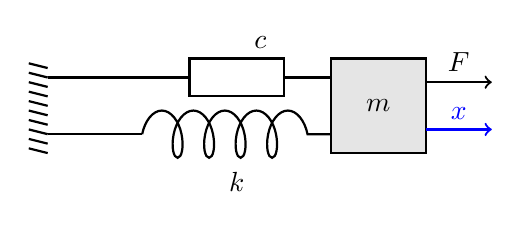
\begin{tikzpicture}[scale=1.2]
        % Draw the wall
        \draw[thick] (-1,.2) -- (0,0.2);
        \draw[thick] (-1,0.8) -- (0,0.8);
        \foreach \y in {0,0.1,...,1.0}
            \draw[thick] (-1,\y) -- (-1.2,\y+0.05);

        % Draw the spring
        \draw[thick,decorate,decoration={coil,aspect=0.5,segment length=4mm,amplitude=3mm}] (0,0.2) -- (2,0.2);

        % Draw the damper
        \draw[thick] (0,0.8) -- (0.5,0.8);
        \draw[thick] (0.5,1.0) rectangle (1.5,0.6);
        \draw[thick] (1.5,0.8) -- (2.0,0.8);

        % Draw the mass
        \draw[thick,fill=gray!20] (2,0) rectangle (3,1.0);

        % Labels
        \node at (2.5,0.5) {$m$};
        \node[above] at (1.25,1.0) {$c$};
        \node[below] at (1,-0.1) {$k$};
        \draw[->,thick,blue] (3.0,0.25) -- ++(0.7,0) node[midway, above] {$x$};
        \draw[->,thick] (3.0,0.75) -- ++(0.7,0) node[midway, above] {$F$};
    \end{tikzpicture}
    \caption{Mass-spring-damper system}
    \label{f:msd}
\end{figure}

Consider the mass-spring-damper system depicted above. The spring exerts a restoring force $-kx$ that is always directed opposite to the displacement $x$ of the mass from equilibrium, while the damper exerts a resistive force $-c\dot{x}$ proportional and opposite to the velocity $\dot{x}$. The external force $F(t)$ acts in the direction of motion. According to Newton's second law, the sum of these forces acting on the mass equals the mass times its acceleration, leading to the equation 
\begin{equation}
m\ddot{x} = F - c\dot{x} - kx 
\end{equation}
Rearranging terms, we obtain the standard form of the equation of motion for the mass-spring-damper system.
\begin{equation}
\ddot{x} + \frac{c}{m}\dot{x} + \frac{k}{m}x = \frac{F}{m}
\end{equation}
This second-order linear differential equation fully describes the dynamic response of the system to any external force $F$. Looking at equation \ref{e:second_order} we can see that $\omega_n = \sqrt{k/m}$ and $\zeta = c/(2\sqrt{mk})$. Furthermore, if we let $F = kf$ we arrive at the same equation as \ref{e:second_order}.

\subsubsection{Attitude Dynamics of a Satellite}

\subsubsection{Pitch Dynamics of an Aircraft}

\subsubsection{Pitch Dynamics of a Rocket}

\hl{include graphic Rocket.png}

\subsection{Characteristic and Particular Solutions to Differential Equations}

The differential equations presented in the previous section can be solved using a variety of methods. The most common methods are the characteristic and particular solution method and the Laplace transform method. The sections below will discuss both methods starting with the characteristic and particular solution method.

\subsubsection{General First Order System}

First the first order system defined above will be solved first. For a first order linear differential equation of the form presented in equation \ref{e:first_order}, the general solution is the sum of the homogeneous (characteristic) solution and a particular solution. The particular solution corresponds to the steady-state response when the forcing function $f$ is constant. In this case assume $f$ is a step function which is just a constant $f_0$. The particular solution $q_p(t)=C$ where $C$ is a constant and thus $\dot{q_p}=\dot{C}=0.$ Plugging this into equation \ref{e:first_order} gives
\begin{equation}
    0 + \sigma q_p = \sigma f_0 
\end{equation}
Thus, the particular solution for a constant input is simply $q_p = f_0$. If the forcing function is not constant then the particular solution will be a function of time and solving for the particular solution will be more difficult. Examples of this include sinusoidal forcing functions or exponentially decaying forcing functions. The solutions to these types of forcing functions can be found in many differential equations textbooks and will not be discussed here for the time being. The homogeneous solution is found by setting the forcing function to zero and solving the resulting equation assuming that $q_h(t)=Ae^{st}$. Thus, the homogeneous equation is
\begin{equation}
    \dot{q_h} + \sigma q_h = Ase^{st} + \sigma Ae^{st} = Ae^{st}(s+\sigma) = 0
\end{equation}
In the equation above the result yields 3 equations that could be equal to zero. The first is $A=0$ which is a trivial solution and thus not considered. The second is $e^{st}=0$ which is never true for any real or complex value of s. The third is $s+\sigma=0$ which is the charactertic equation for the first order system. The solution to this equation yields the characteristic root $s=-\sigma$. Thus, the homogeneous solution is
\begin{equation}
    q_h(t) = Ae^{-\sigma t}
\end{equation}
where A is a constant determined by the initial conditions. The general solution is the sum of the homogeneous and particular solutions
\begin{equation}
    q(t) = q_h(t) + q_p(t) = Ae^{-\sigma t} + f_0
\end{equation}
The constant A can be determined by the initial condition $q(0)=q_0$ which yields
\begin{equation}
    q(0) = A + f_0 = q_0 \implies A = q_0 - f_0
\end{equation}
Thus, the final solution to the first order system is 
\begin{equation}
    q(t) = q_0 - f_0 + Ae^{-\sigma t}
\end{equation}
or more simply
\begin{equation}
    q(t) = f_0 + (q_0 - f_0)e^{-\sigma t}
\end{equation}
In the case of the car example the solution would be
\begin{equation}
    v(t) = \frac{F_0}{c} + \left(v_0 - \frac{F_0}{c}\right)e^{-\frac{c}{m}t}
\end{equation}
noting that $\sigma = c/m$,$F_0 = cf_0$ and $v_0$ is the initial velocity of the car. Typically for these types of systems the initial velocity is zero so the equation simplifies to
\begin{equation}\label{e:first_order_solution}
    v(t) = \frac{F_0}{c}\left(1 - e^{-\frac{c}{m}t}\right)
\end{equation}
which shows that the car will asymptotically approach a steady state velocity of $F_0/c$. This will be plotted later in the time response section for open loop analysis.

\subsubsection{General Second Order Systems}

The solution to second order systems is quite complex given the nature of solving a second order differential equation. The general solution is again the sum of the homogeneous and particular solutions and assume the initial conditions are zero. The major difficulty with second order systems is that the solution to the homogenous characteristic eqaution can be real, repeated or imaginary roots. The roots effect the overall solution and will be discussed later. To start the particular solution is very simple and is again found by assuming a constant forcing function $f_0$ such that $q_p(t)=C$ where $C$ is a constant and thus $\dot{q_p}=\dot{C}=0$ and $\ddot{q_p}=\ddot{C}=0$. Plugging this into equation \ref{e:second_order} gives the eqaution below:

\begin{equation}
    0 + 0 + {\omega_n}^2 q_p = {\omega_n}^2 f_0
\end{equation}
Thus, the particular solution for a constant input is simply $q_p = f_0$. If the forcing function is not constant then the particular solution will be a function of time and solving for the particular solution will be more difficult. Examples of this include sinusoidal forcing functions or exponentially decaying forcing functions. The solutions to these types of forcing functions can be found in many differential equations textbooks and will not be discussed here for the time being. The homogeneous solution is found by setting the forcing function to zero and solving the resulting equation assuming that $q_h(t)=Ae^{st}$. Thus the homogeneous equation is
\begin{equation}
    \begin{matrix}
    \ddot{q_h} + 2\zeta \omega_n \dot{q_h} + {\omega_n}^2 q_h = 0 \\
    A s^2 e^{st} + 2\zeta \omega_n A s e^{st} + {\omega_n}^2 A e^{st} = 0 \\
    Ae^{st}(s^2 + 2\zeta \omega_n s + {\omega_n}^2) = 0
    \end{matrix}
\end{equation}
In the equation above the result yields 3 equations that could be equal to zero. The first is $A=0$ which is a trivial solution and thus not considered. The second is $e^{st}=0$ which is never true for any real or complex value of s. The third is $s^2 + 2\zeta \omega_n s + {\omega_n}^2 = 0$ which is the charactertic equation for the second order system. The solution to this equation yields the characteristic roots which as stated above can have real, repeated or imaginary roots. The characteristic roots are found using the quadratic formula and are given as
\begin{equation}
    s = -\zeta \omega_n \pm \omega_n \sqrt{\zeta^2 - 1}
\end{equation}
The nature of the roots depends on the value of the damping ratio $\zeta$. The three cases are underdamped ($0<\zeta<1$), critically damped ($\zeta=1$), and overdamped ($\zeta>1$). Each case will be discussed below.
\begin{itemize}
    \item {\bf Underdamped ($0<\zeta<1$)}: In this case, the roots are complex conjugates ($s_{12}=-\zeta w_n \pm \omega_d j$), leading to oscillatory behavior. The homogeneous solution is given by:
    \begin{equation}
        q_h(t) = e^{-\zeta \omega_n t} \left( A_1 \cos(\omega_d t) + A_2 \sin(\omega_d t) \right)
    \end{equation}
    where $\omega_d = \omega_n \sqrt{1 - \zeta^2}$ is the damped natural frequency, and $A_1$ and $A_2$ are constants determined by initial conditions.

    \item {\bf Critically Damped ($\zeta=1$)}: In this case, the roots are real and repeated ($s_{12}=-\omega_n$). The homogeneous solution is given by:
    \begin{equation}
        q_h(t) = (A_1 + A_2 t) e^{-\omega_n t}
    \end{equation}

    \item {\bf Overdamped ($\zeta>1$)}: In this case, the roots are real and distinct ($s_{12}=-\zeta \omega_n \pm \omega_n \sqrt{\zeta^2-1}$). The homogeneous solution is given by:
    \begin{equation}
        q_h(t) = A_1 e^{s_1 t} + A_2 e^{s_2 t}
    \end{equation}
\end{itemize}
The general solution is the sum of the homogeneous and particular solutions
\begin{equation}
    q(t) = q_h(t) + q_p(t) = q_h(t) + f_0
\end{equation}
The constants $A_1$ and $A_2$ can be determined by the initial conditions $q(0)=q_0$ and $\dot{q}(0)=\dot{q_0}$. The final solution will depend on the damping ratio $\zeta$ and the initial conditions. For the case where the initial conditions are zero the final solutions for each case are shown below.
\begin{itemize}
    \item {\bf Underdamped ($0<\zeta<1$)}:
    \begin{equation}
        q(t) = f_0 \left( 1 - e^{-\zeta \omega_n t} \left( \cos(\omega_d t) + \frac{\zeta}{\sqrt{1-\zeta^2}} \sin(\omega_d t) \right) \right)
    \end{equation}
    \item {\bf Critically Damped ($\zeta=1$)}:
    \begin{equation}
        q(t) = f_0 \left( 1 - (1 + \omega_n t) e^{-\omega_n t} \right)
    \end{equation}
    \item {\bf Overdamped ($\zeta>1$)}:
    \begin{equation}
        q(t) = f_0 \left( 1 - \frac{s_2 e^{s_1 t} - s_1 e^{s_2 t}}{s_2 - s_1} \right)
    \end{equation}
\end{itemize}
In the case of the mass-spring-damper example, recall that $f_0=F_0/k$, $\omega_n = \sqrt{k/m}$, and $\zeta = c/(2\sqrt{mk})$.

\subsection{Laplace Solutions}

Another method to solve linear differential equations is the Laplace transform method. The Laplace transform converts a time-domain differential equation into an algebraic equation in the s-domain, which can be easier to manipulate and solve. The Laplace domain and algebraic equations are very useful for control system dynamics and every undergraduate controls engineer should learn its fundamentals. The Laplace transform of a function $f(t)$ is defined as 
\begin{equation}
    F(s) = \mathcal{L}\{f(t)\} = \int_0^{\infty} f(t) e^{-st} dt
\end{equation}
where $s$ is a complex variable similar to the $s$ in the $Ae^{st}$ equations discussed earlier. The inverse Laplace transform is given by 
\begin{equation}
    f(t) = \mathcal{L}^{-1}\{F(s)\} = \frac{1}{2\pi j} \lim_{T \to \infty} \int_{\gamma - jT}^{\gamma + jT} F(s) e^{st} ds
\end{equation}
where $\gamma$ is a real number such that all singularities of $F(s)$ are to the left of the line $Re(s) = \gamma$. Note that these integrals are very complex and not typically solved by hand but rather looked up in a table of Laplace transforms. Some common Laplace transforms are shown below
\renewcommand{\arraystretch}{1.5} % Increase row spacing by 1.5x
\begin{table}[H]
\centering
\begin{tabular}{|c|c|c|}
\hline
Time Domain $f(t)$ & Laplace Transform $\mathcal{L}\{f(t)\}$ & Description \\
\hline
$u(t)$ & $\frac{1}{s}$ & Unit step \\
$t$ & $\frac{1}{s^2}$ & Ramp \\
$e^{at}$ & $\frac{1}{s-a}$ & Exponential \\
$sin(at)$ & $\frac{a}{s^2 + a^2}$ & Sine \\
$cos(at)$ & $\frac{s}{s^2 + a^2}$ & Cosine \\
$t^2$ & $\frac{2}{s^3}$ & Quadratic \\
$te^{at}$ & $\frac{1}{(s-a)^2}$ & Repeated Root \\
$e^{at}sin(bt)$ & $\frac{b}{(s-a)^2 + b^2}$ & Underdamped Sine \\
$e^{at}cos(bt)$ & $\frac{s-a}{(s-a)^2 + b^2}$ & Underdamped Cosine \\
$\dot{f}(t)$ & $sF(s) - f(0)$ & First derivative \\
$\ddot{f}(t)$ & $s^2F(s) - sf(0) - \dot{f}(0)$ & Second derivative \\
\hline
\end{tabular}
\caption{Common Laplace transforms}
\end{table}
\renewcommand{\arraystretch}{1} % Reset 
where $u(t)$ is the unit step function where $u(t)=0$ for $t<0$ and $u(t)=1$ for $t\geq0$. The undergraduate student may look at these equations and wonder how exactly these functions are helpful. To illustrate their usefulness the first and second order systems defined above will be solved using the Laplace transform method.

\subsubsection{General First Order Systems}

Taking the Laplace transform of equation \ref{e:first_order} and assuming zero initial conditions gives 
\begin{equation}
    sQ(s) + \sigma Q(s) = \sigma F(s)
\end{equation}
where $Q(s)$ is the Laplace transform of $q(t)$ and $F(s)$ is the Laplace transform of $f(t)$. Rearranging gives the equation below
\begin{equation}
    \frac{Q(s)}{F{s}} = G(s) = \frac{\sigma}{(s+\sigma)}
\end{equation}
The function $G(s)$ is called the transfer function of the system and is a very important function in control systems. The transfer function relates the output of the system $Q(s)$ to the input of the system $F(s)$ in the Laplace domain. The transfer function can be used to analyze the stability and performance of the system. The transfer function can also be used to design controllers for the system which will be discussed later. Let's now assume that the forcing function is a step function such that $f(t)=f_0u(t)$ where $u(t)$ is the unit step function. The Laplace transform of a step function is $F(s)=f_0/s$. Plugging this into the equation above gives
\begin{equation}
    Q(s) = G(s)F(s) = \frac{\sigma}{s+\sigma}\frac{f_0}{s} = \frac{\sigma f_0}{s(s+\sigma)}
\end{equation}
The solution to the equation above can be found by taking the inverse Laplace transform. However, the equation above is not in the standard table of Laplace transforms. Thus partial fraction decomposition is needed to get $Q(s)$ into a form that can be used for inverse Laplace. The equation can be rewritten using partial fractions as
\begin{equation}
    Q(s) = \frac{\sigma f_0}{s(s+\sigma)} = \frac{A}{s} + \frac{B}{s+\sigma}
\end{equation}
where $A$ and $B$ are constants to be determined. Multiplying both sides by the denominator on the left side gives
\begin{equation}
    \sigma f_0 = A(s+\sigma) + Bs
\end{equation}
Setting $s=0$ gives $A=\sigma f_0/\sigma = f_0$. Setting $s=-\sigma$ gives $B=-\sigma f_0/\sigma = -f_0$. Thus, the equation can be rewritten as
\begin{equation}
    Q(s) = \frac{f_0}{s} - \frac{f_0}{s+\sigma}
\end{equation}
Taking the inverse Laplace transform gives
\begin{equation}
    q(t) = f_0 - f_0 e^{-\sigma t} = f_0(1 - e^{-\sigma t})
\end{equation}
substituting back in the values for $\sigma$ and $f_0$ gives
\begin{equation}
    v(t) = \frac{F_0}{c}(1 - e^{-\frac{c}{m}t})
\end{equation}
which is the same solution as derived using the characteristic and particular solution method assuming zero initial conditions as given by equation \ref{e:first_order_solution}.

\subsubsection{General Second Order Systems}

Taking the Laplace transform of equation \ref{e:second_order} and assuming zero initial conditions gives
\begin{equation}
    s^2 Q(s) + 2\zeta \omega_n s Q(s) + {\omega_n}^2 Q(s) = {\omega_n}^2 F(s)
\end{equation}
Rearranging just as before gives the equation below 
\begin{equation}
    \frac{Q(s)}{F(s)} = G(s) = \frac{{\omega_n}^2}{s^2 + 2\zeta \omega_n s + {\omega_n}^2}
\end{equation}
where again $G(s)$ is the transfer function of the system. Let's again assume that the forcing function is a step function such that $f(t)=f_0u(t)$. Plugging the Laplace transform of $F(s)$ just as before gives
\begin{equation}
    Q(s) = G(s)F(s) = \frac{{\omega_n}^2}{s^2 + 2\zeta \omega_n s + {\omega_n}^2}\frac{f_0}{s} = \frac{{\omega_n}^2 f_0}{s(s^2 + 2\zeta \omega_n s + {\omega_n}^2)}
\end{equation}
The solution to the equation above again can be found by taking the inverse Laplace transform. However, again the equation above is not in the standard table of Laplace transforms. Thus partial fraction decomposition is needed to get $Q(s)$ into a form that can be used for inverse Laplace. The equation can be rewritten using partial fractions as
\begin{equation}
    Q(s) = \frac{{\omega_n}^2 f_0}{s(s^2 + 2\zeta \omega_n s + {\omega_n}^2)} = \frac{A}{s} + \frac{Bs + C}{s^2 + 2\zeta \omega_n s + {\omega_n}^2}
\end{equation}
where $A$, $B$ and $C$ are constants to be determined. Multiplying both sides by the denominator on the left side gives
\begin{equation}
    {\omega_n}^2 f_0 = A(s^2 + 2\zeta \omega_n s + {\omega_n}^2) + (Bs + C)s
\end{equation}
Setting $s=0$ gives $A={\omega_n}^2 f_0/{\omega_n}^2 = f_0$. Setting $s=j\omega_n(-\zeta + \sqrt{\zeta^2 - 1})$ and $s=j\omega_n(-\zeta - \sqrt{\zeta^2 - 1})$ gives two equations that can be solved simultaneously to find $B$ and $C$. The final results are $B=-f_0$ and $C=-2\zeta \omega_n f_0$. Thus, the equation can be rewritten as
\begin{equation}
    Q(s) = \frac{f_0}{s} - \frac{f_0 s + 2\zeta \omega_n f_0}{s^2 + 2\zeta \omega_n s + {\omega_n}^2}
\end{equation}
The first term of the equation is simply the Laplace transform of a step function. The second term can be solved using the table of Laplace transforms. The final solution depends on the value of the damping ratio $\zeta$ just as before. The final solutions for each case assuming zero initial conditions are shown below. It is left to the reader to verify that these solutions match those derived using the characteristic and particular solution method. The underdamped solution is solved by completing the square in the denominator and using the Laplace transform of the underdamped sine and cosine functions. The critically damped and overdamped solutions are solved using the Laplace transforms of repeated roots and real distinct roots respectively.
\begin{itemize}
    \item {\bf Underdamped ($0<\zeta<1$)}:
    \begin{equation}
        q(t) = f_0 \left( 1 - e^{-\zeta \omega_n t} \left( \cos(\omega_d t) + \frac{\zeta}{\sqrt{1-\zeta^2}} \sin(\omega_d t) \right) \right)
    \end{equation}
    \item {\bf Critically Damped ($\zeta=1$)}:
    \begin{equation}
        q(t) = f_0 \left( 1 - (1 + \omega_n t) e^{-\omega_n t} \right)
    \end{equation}
    \item {\bf Overdamped ($\zeta>1$)}:
    \begin{equation}
        q(t) = f_0 \left( 1 - \frac{s_2 e^{s_1 t} - s_1 e^{s_2 t}}{s_2 - s_1} \right)
    \end{equation}
\end{itemize}
Notice again that the solutions are the same as those derived using the characteristic and particular solution method assuming zero initial conditions. It is possible that the undergraduate engineer still does not see the usefulness of the Laplace transform method. The true power of the Laplace transform method is in the transfer function. The transfer function can be used to analyze the stability and performance of the system as well as design controllers for the system which will be discussed in the sections below.

\subsection{Open Loop Time Response}

Now that the solutions to the first and second order systems have been derived using both the characteristic and particular solution method as well as the Laplace transform method, the time response of these systems can be analyzed. The time response of a system is the output of the system as a function of time given a specific input. The time response can be used to analyze the stability and performance of the system. 

\subsubsection{Velocity Response of a Car}

First, let's plot the time response of the first order system given by equation \ref{e:first_order_solution}. The parameters for the system are chosen to be $F_0=1000~N$, $c=50~Ns/m$, and $m=1000~kg$. The initial velocity is assumed to be zero. In order to show the time response however, 3 different curves will be placed on the graph. The first will be the analytic solution to the first order system, the second is the Laplace transform solution using the control systems toolbox in Python and the last is the numerical integration of the equations of motion. The python code used to generate this is shown in the Figure below and also available on \href{https://github.com/cmontalvo251/Python/blob/master/controls/first_order_system.py}{GitHub}.
\begin{figure}[H]
\centering
\includegraphics[width=0.7\textwidth]{Figures/first_order_code.png}
\caption{Python code to generate time response of first order system}
\label{f:first_order_code}
\end{figure}
Note the code is commented to help the reader understand what is happening. Note the benefit of using the control systems toolbox in Python. The time response can be generated by first creating the transfer function and then applying a step to the transfer function. This will come in handy later when it is necessary to apply a control system to the transfer function before inversing back to the time domain. The numerical integration is also useful when the equations of motion are known and the control system designer wants to work in the time doman rather than the laplace domain. Both have their pros and cons. The numerical integration is done using the scipy.integrate.odeint function which is a simple way to numerically integrate ordinary differential equations. The results of the time response are shown in Figure \ref{f:first_order_response}.
\begin{figure}[H]
    \centering
    \includegraphics[width=0.7\textwidth]{Figures/first_order_response.png}
    \caption{Time response of first order system}
    \label{f:first_order_response}
\end{figure}
\noindent The time response shows that the velocity of the car asymptotically approaches a steady state value of $F_0/c = 20~m/s$. The time constant of the system is $\tau = m/c = 20~s$. The time constant is the time it takes for the system to reach 63.2\% of its steady state value. The settling time $T_s=4\tau$ is the time the system takes to get within 2\% of its final value. In this case that is $80~s$. The time response can be used to analyze the stability and performance of the system. In this case, the system is stable and the performance is acceptable given the parameters chosen. 

\subsubsection{Position of a Mass Spring Damper}

\subsubsection{Attitude of a Satellite}

\subsubsection{Pitch Response of an Aircraft}

\subsubsection{Pitch Response of a Rocket}

\subsection{Stability}

\subsubsection{Roots of the Characteristic Equation}

\subsubsection{Poles of the Transfer Function}

\subsection{Proportional Derivative Integral Control}

\subsubsection{Bang Bang Control of a Satellite}

\subsubsection{Proportional Control of a Satellite}

\hl{include graphic of Feedback.png}

\subsubsection{Proportional Derivative Control of a Satellite}

\subsubsection{Proportional Control of a Car}

\subsubsection{Proportional Integral Control of a Car}

\subsubsection{Proportional Integral Derivative Control of an Aircraft}

\subsection{Inner and Outer Loop Control of an Aircraft}

\subsubsection{Velocity Control}

\subsubsection{Altitude Control}

\subsubsection{Roll Angle Control}

\subsubsection{Heading Angle Control of a Car}

\subsubsection{Heading Angle Control of an Airplane}

\subsubsection{Waypoint COntrol of a Car}

\subsubsection{Waypoint Control of an Airplane}

\subsection{Lyapunov Control}

\subsection{Sliding Mode Control}

\subsection{Adaptive Control}

\subsection{Controllability}

Controllability is formally stated as a system where any initial
state $x(0)=x_0$ and final state $x_1,t_1>0$, there exists a piecewise
continuous input $u(t)$ such that $x(t_1)=x_1$. 
For a fixed wing aircraft the system has 12 states with 8 dynamic
modes and 4 zero or rigid body modes. For a fixed wing aircraft the system has 12 states with 8 dynamic
modes and 4 zero or rigid body modes. A conventional aircraft has 4
controls to control these 12 modes. The easiest way to test the 
controllability of a system  is to compute the
controllability matrix. However, the controllability matrix must be
computed using a linearized model such that
$\dot{\vec{x}}=A\vec{x}+B\vec{u}$. In order to do this the aircraft
must be in equilibrium. For this example the aircraft is
set with an initial velocity of $20~m/s$ at an altitude of
$200~m$. The altitude command is set to $200~m$ and the heading
command is set to zero. Given the zero heading angle command and the
symmetry of the configurations investigated the rudder and aileron
commands are set to zero. Thus, only the thrust and elevator controls
are activated for the trimming procedure. Each configuration is
simulated for 200 seconds or until the derivatives of all states
except $\dot{x}$ are within a required tolerance. Using this
equilibrium point a linear model can be computed by using forward
finite differencing assuming that the
aircraft model is put in the form $\dot{\vec{x}} = F(\vec{x},\vec{u})$.
\begin{equation}
\dot{\vec{\delta x}} = \frac{F(\vec{x_0}+\Delta \vec{x_0},\vec{u_0})-F(\vec{x_0},\vec{u_0})}{\Delta
  \vec{x}}\vec{\delta x} + \frac{F(\vec{x_0},\vec{u_0}+\Delta
  \vec{u})-F(\vec{x_0},\vec{u_0})}{\Delta \vec{u}}\vec{\delta u}
\end{equation}
This linear model is the classic linear model where
$\dot{\vec{\delta x}}=A\vec{\delta{x}}+B\vec{\delta{u}}$. Using this linear model, the
controllability matrix can be computed as
\begin{equation}
W_C = [B~AB~A^2B~A^3B~...~A^{N-1}B]
\end{equation}
where N is the number of states in the system. With the controllability
matrix formulated, the rank of the matrix is computed. If the
$rank(W_C)=N$ the system is said to be controllable.

